\documentclass[oneside,12pt,fancychapters]{scrbook} %%%%mine
\usepackage[utf8]{inputenc}
\usepackage{minitoc} %to get mini table of contents for each chapter
\usepackage{hyperref} %hyperlinks

\usepackage{graphicx}
\usepackage{subcaption}
\usepackage{subfigure}


\title{Roombee Manual}
\author{Marcus Futterlieb}
\date{20.01.2016}

\pdfinfo{%
  /Title    (roombee manual)
  /Author   (Marcus Futterlieb)
  /Creator  (Marcus Futterlieb) 
  /Producer (Marcus Futterlieb)
  /Subject  (mobile robotics)
  /Keywords (mobile robotics, drive by odometry, diy robot)
}

\begin{document}
\dominitoc
\maketitle

\tableofcontents

\chapter{Disclaimer}
This software has been developed to allow curious owners of a iRobot Roomba 500 series to gather some experience in the domain of mobile robotics. 
A serious help in the development was "The MATLAB Toolbox for the iRobot Create" which can be found \href{http://www.usna.edu/Users/weapsys/esposito/roomba-matlab.php}{here}.
The author can not be held responsible for any damage caused directly or indirectly by the software. 


\chapter{Prerequisites and Requirements}
In order to use this software you need a few things.
Apart from the robot (you can find cheap offers of used robots on ebay, or your local equivalent) and a laptop you will need:
\begin{itemize}
  \item A working Matlab version (all above 2012b should work fine)
  \item A serial connection (USB to serial is sufficient, however you can find offers that provide a serial to blue-tooth connection)
  \item (optional) Some kind of small platform you can mount on the robot to provide a more reliable base for your laptop
\end{itemize}

\chapter{Get the Robot operational}


\begin{figure}
\centering     %%% not \center
\subfigure[Figure B]{\label{fig:b}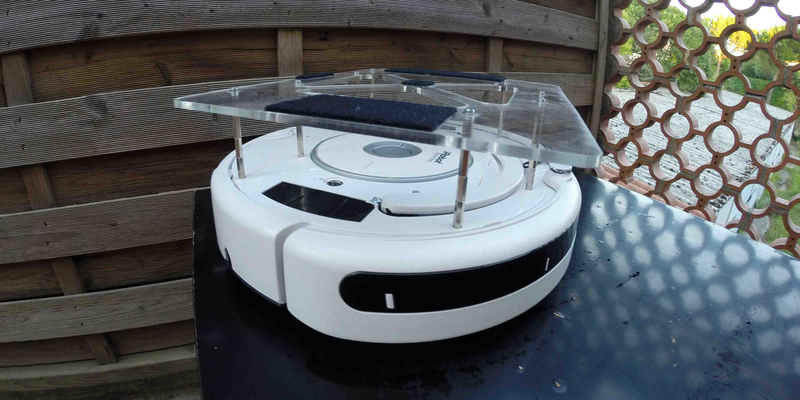
\includegraphics[width=0.45\textwidth]{media/resized/0.png}}
\subfigure[Figure B]{\label{fig:b}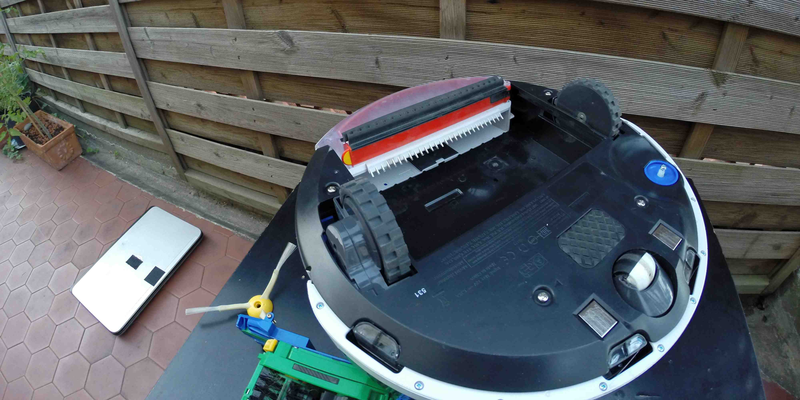
\includegraphics[width=0.45\textwidth]{media/resized/1.png}}
\subfigure[Figure B]{\label{fig:b}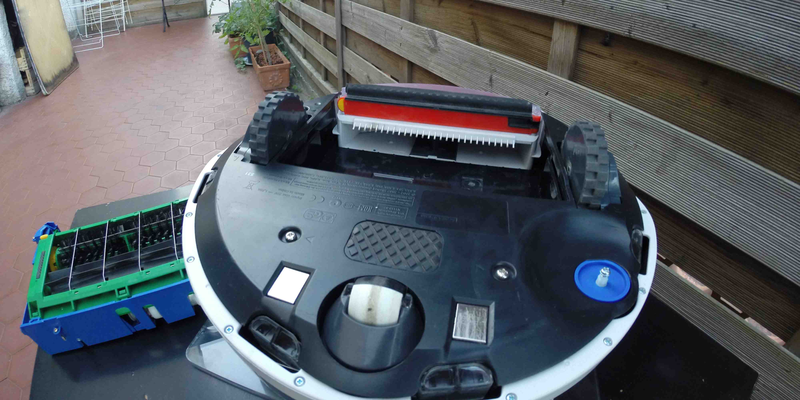
\includegraphics[width=0.45\textwidth]{media/resized/2.png}}
\subfigure[Figure B]{\label{fig:b}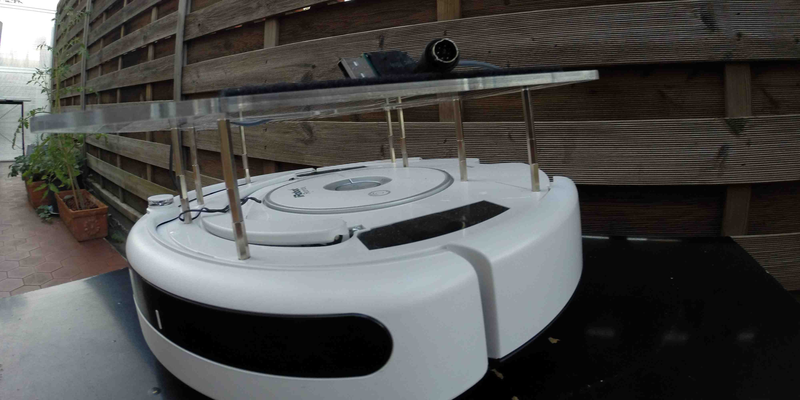
\includegraphics[width=0.45\textwidth]{media/resized/3.png}}
\subfigure[Figure B]{\label{fig:b}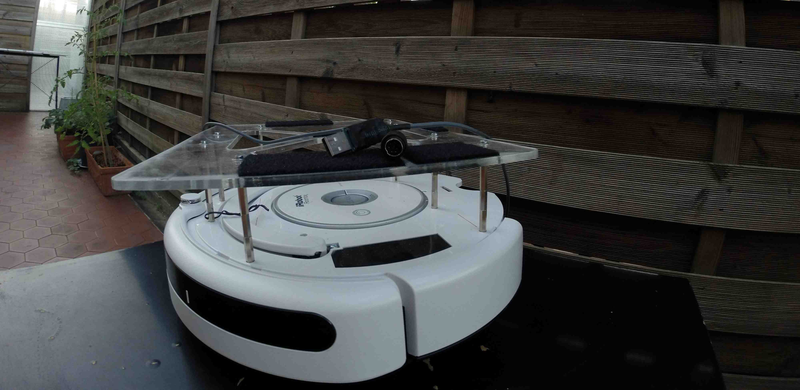
\includegraphics[width=0.45\textwidth]{media/resized/4.png}}
\subfigure[Figure B]{\label{fig:b}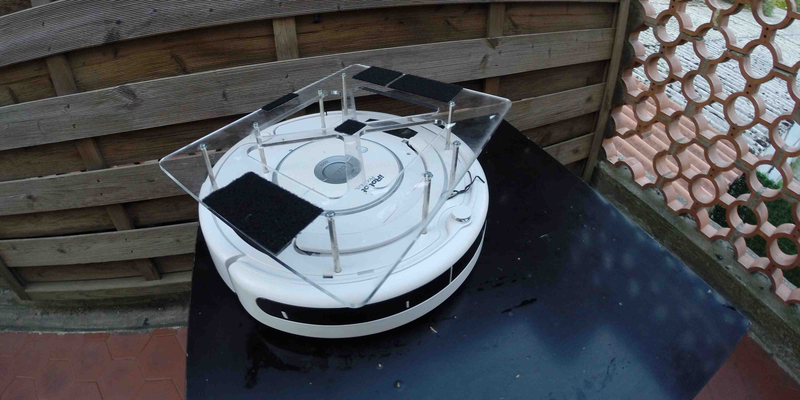
\includegraphics[width=0.45\textwidth]{media/resized/5.png}}
\caption{How to prepare the iRbobot Roomba}
\label{fig:setup_1}
\end{figure}

\begin{figure}
\centering     %%% not \center
\subfigure[Figure B]{\label{fig:b}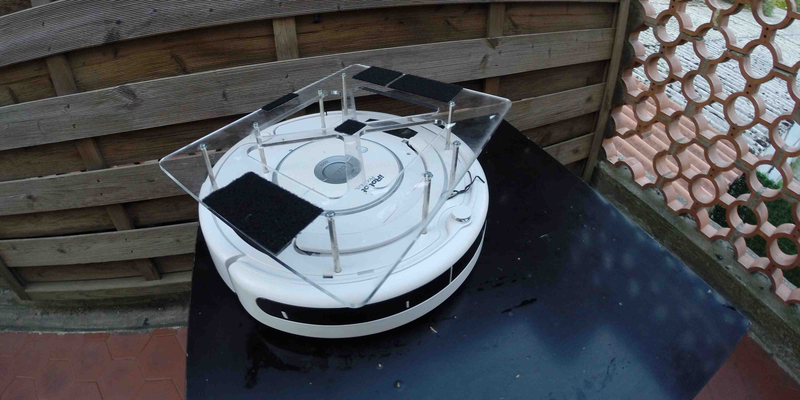
\includegraphics[width=0.45\textwidth]{media/resized/6.png}}
\subfigure[Figure B]{\label{fig:b}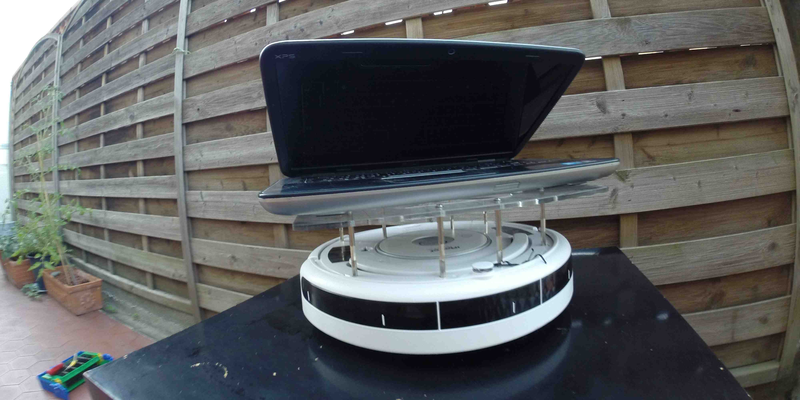
\includegraphics[width=0.45\textwidth]{media/resized/7.png}}
\subfigure[Figure B]{\label{fig:b}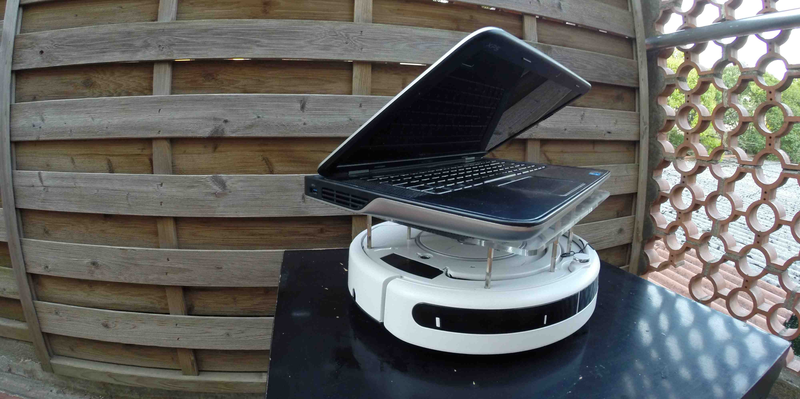
\includegraphics[width=0.45\textwidth]{media/resized/8.png}}
\subfigure[Figure B]{\label{fig:b}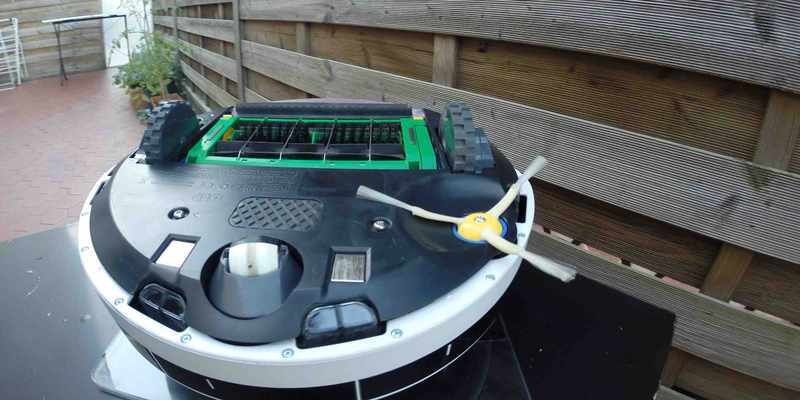
\includegraphics[width=0.45\textwidth]{media/resized/9.png}}
\subfigure[Figure B]{\label{fig:b}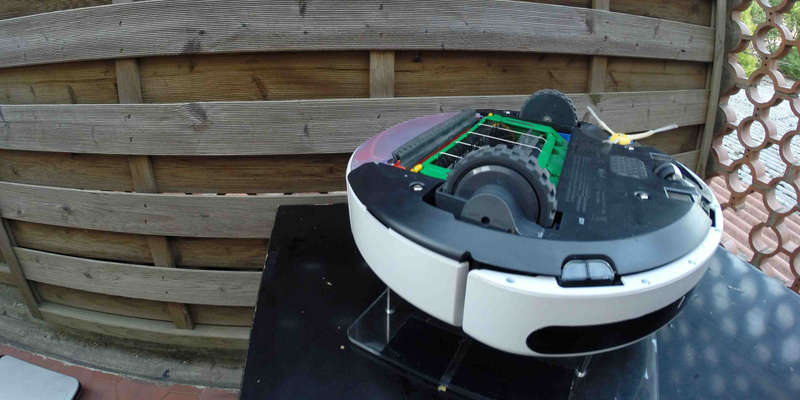
\includegraphics[width=0.45\textwidth]{media/resized/10.png}}
\subfigure[Figure B]{\label{fig:b}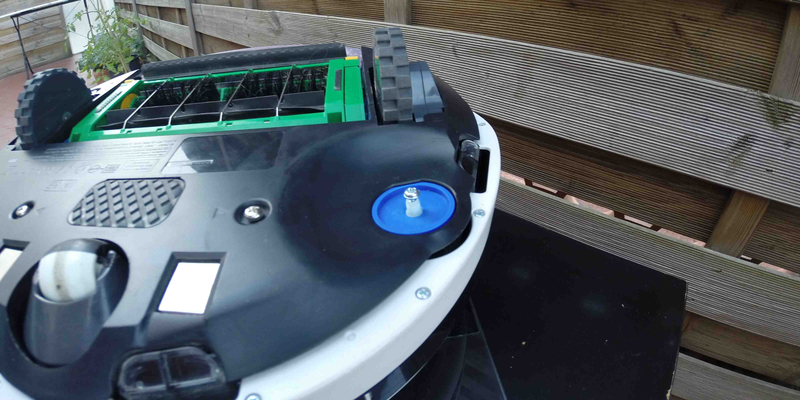
\includegraphics[width=0.45\textwidth]{media/resized/11.png}}
\caption{Extract of video sequence~\cite{???!!!} - dynamic obstacles (b)}
\label{fig:video_dynamic_2}
\end{figure}

\begin{figure}
\centering     %%% not \center
\subfigure[Figure B]{\label{fig:b}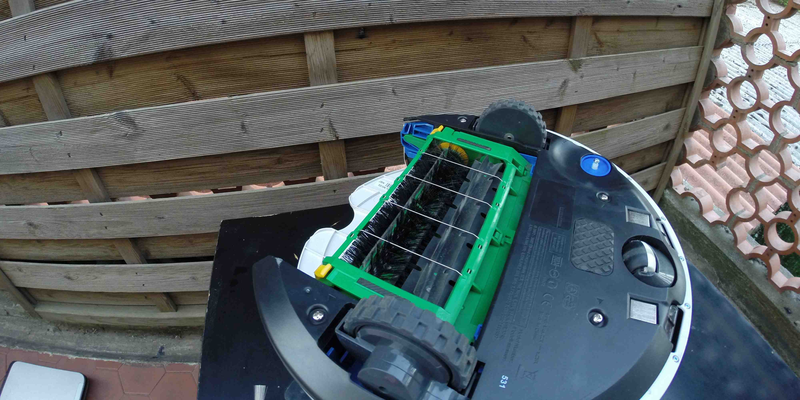
\includegraphics[width=0.45\textwidth]{media/resized/12.png}}
\subfigure[Figure B]{\label{fig:b}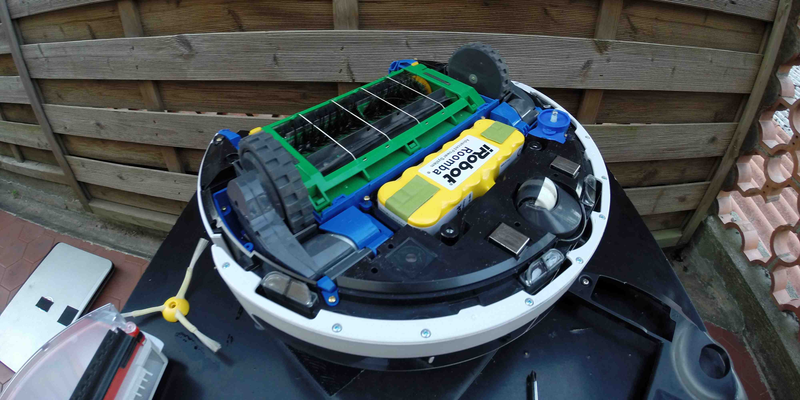
\includegraphics[width=0.45\textwidth]{media/resized/13.png}}
\subfigure[Figure B]{\label{fig:b}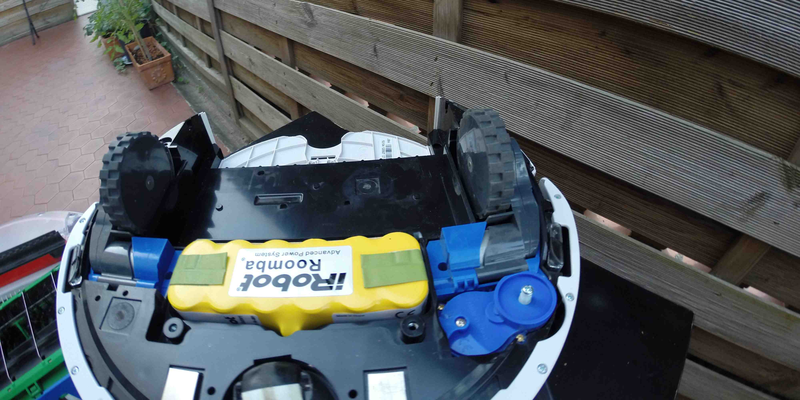
\includegraphics[width=0.45\textwidth]{media/resized/14.png}}
\caption{Extract of video sequence~\cite{???!!!} - dynamic obstacles (b)}
\label{fig:video_dynamic_2}
\end{figure}


\chapter{How to use the Code}
\chapter{How to create the Light Graffiti Effect}
The tool used for post processing the video material is \href{https://kdenlive.org/}{Kdenlive}.
It should be accessible through the apt-get command.
Once installed it handles much like any other video editing software.
The effect you are looking for is called "Light Graffiti" and can be found under:\\
\textbf{Effect List/Misc/ Light Graffiti} \\
You have to choose your parameters so that the brightest point in the video is the light source in the center of the robot.
A head lamp for camping should be sufficient. 


\vspace {0.5cm}

Examples can be found at:

\begin{itemize}
  \item \href{https://youtu.be/hPpPM0kasyk}{Youtube video of a Roomba following a certain letter sequence indoors}
  \item \href{https://youtu.be/g-6yrYu4PUs}{Youtube video of a Roomba following a certain letter sequence outdoors}
\end{itemize}




\end{document}
